\documentclass[12pt]{article}
\usepackage[active,
            generate=Math_514_Definitions,
            %extract-cmd={section},
            extract-env={definition,algorithm}]{extract}

\begin{extract*}
  \usepackage{amsthm}
  \usepackage{amsfonts, amsmath}
  \usepackage[dvipsnames]{xcolor}
  %\newtheorem{theorem}{Theorem}
  \theoremstyle{definition}
  \definecolor{Tm}{rgb}{0,0,0.80}
  %\newtheorem{definition}{Definition}
  \newtheorem{definition}{\color{NavyBlue}{\textbf{Definition}}}
  %\newtheorem{example}{Example}
  	\usepackage{bm}
	\newcommand{\e}{\epsilon}
	%\newcommand{\d}{\delta}
	\newcommand{\D}{\Delta}
	\newcommand{\R}{\mathbb{R}}
	\newcommand{\Z}{\mathbb{Z}}
	\usepackage{mathtools}
	\DeclarePairedDelimiterX{\inp}[2]{\langle}{\rangle}{#1, #2}
	\newcommand{\norm}[1]{\lVert#1\rVert}
	\newcommand{\x}{\bm{x}}
	\newcommand{\xib}{\bm{\xi}}
	\usepackage{mathrsfs}
	\usepackage{algpseudocode,algorithm,algorithmicx}
	\algnewcommand\algorithmicforeach{\textbf{for each}}
	\algdef{S}[FOR]{ForEach}[1]{\algorithmicforeach\ #1\ \algorithmicdo}
	\newcommand*\Let[2]{\State #1 $\gets$ #2}
\end{extract*}

\usepackage{algpseudocode,algorithm,algorithmicx}
%\usepackage{amsfonts, amsmath}
\usepackage{amssymb, geometry}
\usepackage{scalefnt}
\usepackage{setspace}
\usepackage{color,hyperref}
%\usepackage{epsfig,subfigure,morefloats}
\usepackage{natbib}
\usepackage{dsfont}
\usepackage{color,hyperref}
\usepackage{epstopdf}
%\usepackage{amsthm}
\usepackage{amssymb}
%\usepackage{subcaption}
\usepackage{graphicx}
\usepackage{booktabs,siunitx}
\usepackage{bm}
\usepackage[section]{placeins}
%\usepackage{hypcap}
\usepackage{afterpage}


\setcounter{MaxMatrixCols}{10}

\providecommand{\u}[1]{\protect\rule{.1in}{.1in}}
\providecommand{\u}[1]{\protect\rule{.1in}{.1in}}
\newtheorem{theorem}{\color{ForestGreen}{\textbf{Theorem}}}
\newtheorem{acknowledgement}[theorem]{Acknowledgement}
%\newtheorem{algorithm}[theorem]{Algorithm}
\newtheorem{axiom}[theorem]{Axiom}
\newtheorem{case}[theorem]{Case}
\newtheorem{claim}{\color{JungleGreen}Claim}
\newtheorem{conclusion}[theorem]{Conclusion}
\newtheorem{condition}[theorem]{Condition}
\newtheorem{conjecture}{Conjecture}
\newtheorem{corollary}{Corollary}
\newtheorem{criterion}[theorem]{Criterion}
% \newtheorem{definition}{Definition}
% \theoremstyle{definition}
\newtheorem{example}{\color{WildStrawberry}Example}
\newtheorem{exercise}{\color{YellowOrange}Exercise}
\newtheorem{lemma}{Lemma}
\newtheorem{notation}[theorem]{Notation}
\newtheorem{problem}[theorem]{Problem}
\newtheorem{proposition}{Proposition}
\newtheorem{remark}{Remark}
\theoremstyle{definition}
%\newtheorem{solution}[theorem]{Solution}
\newtheorem{solution}{\color{Goldenrod}Solution}
\newtheorem{summary}[theorem]{Summary}
\geometry{left=1in,right=1in,top=1in,bottom=1in}
%\newenvironment{proof}[1][Proof]{\noindent\textbf{#1.} }{\ \rule{0.5em}{0.5em}}
%\hypersetup{pdftex,colorlinks=true,allcolors=black,citecolor=black}

%\usepackage{floatrow}
\usepackage{float}
\usepackage{indentfirst}

% \algrenewcommand\alglinenumber[1]{
%     {\sf\footnotesize\addfontfeatures{Colour=888888,Numbers=Monospaced}#1}}
% \algrenewcommand\algorithmicrequire{\textbf{Precondition:}}
%\algrenewcommand\algorithmicensure{\textbf{Postcondition:}}


\DeclareMathOperator*{\argmax}{arg\,max}
\DeclareMathOperator*{\argmin}{arg\,min}

\graphicspath{{./figures/}}

\usepackage{listings}
\usepackage{subcaption} 
\usepackage[toc,page]{appendix}
%\usepackage[extendedchars]{grffile}

\usepackage{mathpazo} % math & rm
\linespread{1.05}        % Palatino needs more leading (space between lines)
\usepackage[scaled]{helvet} % ss
\usepackage{courier} % tt
\normalfont
\usepackage[T1]{fontenc}

%% Math commands
% \newcommand{\e}{\epsilon}
% %\newcommand{\d}{\delta}
% \newcommand{\D}{\Delta}
% \newcommand{\R}{\mathbb{R}}
% \newcommand{\Z}{\mathbb{Z}}
% \usepackage{mathtools}
% \DeclarePairedDelimiterX{\inp}[2]{\langle}{\rangle}{#1, #2}
% \newcommand{\norm}[1]{\lVert#1\rVert}
% \newcommand{\x}{\bm{x}}
% \newcommand{\xib}{\bm{\xi}}
% \usepackage{mathrsfs}


\title{Numerical Analysis Lecture Notes}
\author{Rebekah Dix}
\begin{document}
\maketitle
\tableofcontents
\newpage 

\section{Results from Real Analysis}
\begin{theorem}(The Mean Value Theorem)
Suppose $f$ is a real-valued function, defined and continuous on the closed interval $[a,b] \in \R$ and $f$ differentiable on the open interval $(a,b)$. Then there exists a number $\xi \in (a,b)$ such that
\begin{equation}
	f(b) - f(a) = f'(\xi) (b - a)
\end{equation}
\end{theorem}

\begin{theorem}(Taylor's Theorem)
Suppose that $n$ is a nonnegative integer, and $f$ is a real-valued function, defined and continuous on the closed interval $[a,b]$ of $\R$, such that the derivatives of $f$ of order up to and including $n$ are defined and continuous on the closed interval $[a,b]$. Suppose further that $f^{(n)}$ is differentiable on the open interval $(a,b)$. Then, for each value of $x \in [a,b]$, there exists a number $\xi = \xi(x)$ in the open interval $(a,b)$ such that 
\begin{equation}
	f(x) = f(a) + (x-a)f'(a) + \cdots + \frac{(x-a)^n}{n!} f^{(n)}(a) + \frac{(x-a)^{n+1}}{(n+1)!} f^{(n+1)}(\xi)
\end{equation}
\end{theorem}

\section{Solution of equations by iteration}

\subsection{Simple Iteration}
\begin{theorem}(Existence of Root)\label{zeroexists}
Let $f$ be a real-valued function, defined and continuous on a bounded closed interval $[a,b]$ of the real line. Assume further, that $f(a)f(b) \leq 0$; then, there exists $\xi$ in $[a,b]$ such that $f(\xi) = 0$.
\end{theorem}
\begin{proof}
The condition $f(a)f(b) \leq 0$ implies that $f(a)$ and $f(b)$ have opposite signs, or one of them is $0$. If either $f(a)$ or $f(b)$ is $0$, then we've found a root. Suppose that both endpoints are non-zero (in which case they have opposite signs). In this case, $0$ must belong to the open interval whose endpoints are $f(a)$ and $f(b)$. The intermediate value theorem gives the existence of a root in the open interval $(a,b)$. Thus, in both cases, a zero is guaranteed. 
\end{proof}

\begin{itemize}
\item The converse of Theorem \ref{zeroexists} is clearly false.
\end{itemize}

\begin{theorem}(Brouwer's Fixed Point Theorem)
Suppose that $g$ is a real-valued function, defined and continuous on a bounded closed interval $[a,b]$ of the real line, and let $g(x) \in [a,b]$ for all $x \in [a,b]$. Then, there exists $\xi \in [a,b]$ such that $\xi = g(\xi)$. $\xi$ is called a fixed point of the function $g$. 
\end{theorem}
\begin{proof}
Define a function $f(x) = x - g(x)$. If we find a root $\xi$ of $f$, then $\xi$ is a fixed point of $g$. Then,
\begin{equation}
f(a)f(b) = (a - g(a))(b-g(b)) \leq 0
\end{equation}
By assumption, $a \leq g(a), g(b) \leq b$. Therefore, the first term is negative and the second term is positive. Therefore, $f(a)f(b) \leq 0$. By Theorem \ref{zeroexists}, there exists a $\xi \in [a,b]$ such that $f(\xi)=0$. Then, for this $\xi$, $g(\xi) = \xi$.
\end{proof}

\begin{definition}(Simple Iteration)
Suppose that $g$ is a real-valued function, defined and continuous on a bounded closed interval $[a,b]$ of the real line, and let $g(x) \in [a,b]$ for all $x \in [a,b]$. Given that $x_0 \in [a,b]$, the recursion defined by 
\begin{equation}
x_{k+1} = g(x_k)
\end{equation}
is called simple iteration; the numbers $x_k$, $k \geq 0$, are referred to as iterates.
\end{definition}

\begin{itemize}
\item If this sequence converges, the limit must be a fixed of $g$, since $g$ is continuous on a closed interval. Note that
\begin{equation}
\xi = \lim_{k \to \infty} x_{k+1} = \lim_{k \to \infty} g(x_k) = g\left( \lim_{k \to \infty} x_k \right) = g(\xi)
\end{equation}
\end{itemize}

\begin{definition}(Contraction)
Let $g$ be a real-valued function, defined and continuous on a bounded closed interval $[a,b]$ of the real line. Then, $g$ is said to be a contraction on $[a,b]$ if there exists a constant $L$ such that $0<L<1$ and 
\begin{equation}
|g(x)-g(y)| \leq L|x-y| \quad \forall x,y \in [a,b]
\end{equation}
\end{definition}

\begin{theorem}(Contraction Mapping Theorem)
Suppose that $g$ is a real-valued function, defined and continuous on a bounded closed interval $[a,b]$ of the real line, and let $g(x) \in [a,b]$ for all $x \in [a,b]$. Suppose $g$ is a contraction on $[a,b]$. Then, $g$ has a unique fixed point $\xi$ in the interval $[a,b]$. Moreover, the sequence $(x_k)$ defined by simple iteration converges to $\xi$ as $k \to \infty$ for any starting value $x_0$ in $[a,b]$. 

Let $\epsilon > 0$ be a certain tolerance, and let $k_0 (\epsilon)$ denote the smallest positive integer such that $x_k$ is no more than $\epsilon$ away from the fixed point $\xi$ (i.e. $|x_k - \xi| \leq \epsilon$) for all $k \geq k_0 (\epsilon)$. Then,
\begin{equation}
k_0 (\epsilon) \leq \left\lfloor \frac{\ln|x_1 - x_0| - \ln(\epsilon (1 - L))}{\ln (1 / L)}\right\rfloor + 1
\end{equation}
\end{theorem}

\begin{proof}
Let $E_k = |x_k - \xi|$ be the error at $k$. Then 
\begin{align*}
|x_{k+1} - \xi| &= |g(x_k) - g(\xi)| \tag{definition of $g$ and $\xi$ a fixed point}\\
&< L |x_k - \xi| \tag{$g$ a contraction}
\end{align*}
Therefore by induction
\begin{equation}
	E_{k} \leq L^k E_0
\end{equation}
Since $L < 1$, $L^k \to 0$ as $k \to \infty$, so that $\lim_{k \to \infty} |x_k - \xi| = 0$. 
\end{proof}

\begin{theorem}(Contraction Mapping Theorem when Differentiable)
Suppose that $g$ is a real-valued function, defined and continuous on a bounded closed interval $[a,b]$ of the real line, and let $g(x) \in [a,b]$ for all $x \in [a,b]$. Let $\xi= g(\xi) \in [a,b]$ be a fixed point of $g$ (the existence of this point is guaranteed by Brouwer's fixed point theorem). Assume $g$ has a continuous derivative in some neighborhood of $\xi$ with $|g'(\xi)| < 1$. Then the sequence $(x_k)$ defined by simple iteration $x_{k+1} = g(x_k)$, $k \geq 0$, converges to $\xi$ as $k \to \infty$, provided that $x_0$ is close to $\xi$. 
\end{theorem}

\begin{definition}(Stable, Unstable Fixed Point)
Suppose that $g$ is a real-valued function, defined and continuous on a bounded closed interval $[a,b]$ of the real line, and let $g(x) \in [a,b]$ for all $x \in [a,b]$, and let $\xi$ denote a fixed point of $g$. $\xi$ is a stable fixed point of $g$ if the sequence $(x_k)$ defined by the iteration $x_{k+1} = g(x_k)$, $k\geq 0$, converges to $\xi$ whenever the starting value $x_0$ is sufficiently close to $\xi$. Conversely, if no sequence $(x_k)$ defined by this iteration converges to $\xi$ for any starting value $x_0$ close to $\xi$, except for $x_0 = \xi$, then we say that $\xi$ is an unstable fixed point of $g$. 
\end{definition}
\begin{itemize}
	\item With this definition, a fixed point may be neither stable nor unstable.
	\item If $|g'(\xi)| < 1$, then $\xi$ is a stable fixed point (provided $g$ is continuous, differentiable etc.)
\end{itemize}

\begin{theorem}(Unstable Fixed Points)
	Suppose that $\xi = g(\xi)$, where the function $g$ has a continuous derivative in some neighborhood of $\xi$, and let $|g'(\xi)| > 1$ (thus $\xi$ is an unstable fixed point). Then the sequence $(x_k)$ defined by simple iteration $x_{k+1} = g(x_k)$, $k \geq 0$, does not converge to $\xi$ from any starting value $x_0$, $x_0 \neq \xi$. 
\end{theorem}

\begin{definition}(Rate of Convergence)
Suppose $\xi = \lim_{k \to \infty} x_k$. Define $E_k = |x_k - \xi|$.
\end{definition}
\begin{itemize}
\item The sequence $(x_k)$ converges to $\xi$ linearly if there exists a number $\mu \in (0,1)$ such that 
\begin{equation}
\lim_{k \to \infty} \frac{E_{k+1}}{E_k} = \mu
\end{equation}
\item The sequence $(x_k)$ converges to $\xi$ superlineraly if $\mu = 0$. That is, the sequence of $\mu_k$ generated at each step $\rightarrow 0$ as $k \rightarrow \infty$.
\item The sequence $(x_k)$ converges to $\xi$ with order $q$ if there exists a $\mu > 0$ such that
\begin{equation}
\lim_{k \to \infty} \frac{E_{k+1}}{E_k^q} = \mu
\end{equation}
In particular, if $q=2$, then the sequence converges quadratically.
\end{itemize}

\subsection{Newton's Method}

\begin{definition}(Newton's Method)
Newton's method for the solution of $f(x) = 0$ is defined by 
\begin{equation}
	x_{k+1} = x_k - \frac{f(x_k)}{f'(x_k)}
\end{equation}
\end{definition}

Geometrically, $(x_{n+1}, 0)$ is the intersection of the $x$-axis and the tangent of the graph of $f$ at $(x_n, f(x_n))$. 

\begin{figure}[H]
	\begin{center}
		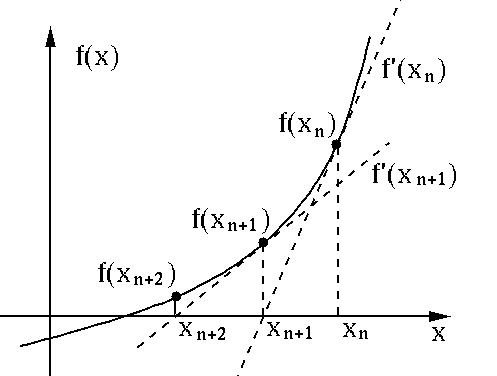
\includegraphics[scale=.5]{newton_method.png}
	\end{center}
	\caption{Geometric Interpretation of Newton's Method in $\R$}
\end{figure}

Intuitively, the fixed points of this iteration $g$ will be stable. 

We can show that $|g'(\xi)| < 1$. 
\begin{align*}
	g'(x) &= 1 - \frac{f'\cdot f' - f\cdot f''}{(f')^2} \\
	&= 1 - \left( 1 - \frac{f(x)\cdot f''(x)}{(f'(x))^2}\right) \\
	&= \frac{f(x)\cdot f''(x)}{(f'(x))^2}
\end{align*}
Therefore
\begin{equation}
	|g'(\xi)| = \left\vert \frac{f(\xi)\cdot f''(\xi)}{(f'(\xi))^2} \right\vert = 0 < 1
\end{equation}

\begin{theorem}(Convergence of Newton's Method)
Suppose that $f$ is a continuous real-valued function with continuous second derivative $f''$ defined on the closed interval $I_\delta = [\xi - \delta, \xi + \delta]$, $\delta > 0$, such that $f(\xi) = 0$ and $f''(\xi) \neq 0$. Additionally suppose that there exists a positive constant $A$ such that 
\begin{equation}
	\frac{|f''(x)|}{|f'(y)|} \leq A \quad \forall x,y, \in I_\delta
\end{equation}
If initially
\begin{equation}
	|\xi - x_0| \leq h = \min(\delta, \frac{1}{A})
\end{equation}
then the sequence $(x_k)$ defined by Newton's method converges quadratically to $\xi$. 
\end{theorem}

\begin{proof}
We first compute the Taylor expansion of $f(\xi)$, expanding about the point $x_k \in I_\delta$, where $|\xi - x_k| \leq h = \min(\delta, \frac{1}{A})$. Thus
\begin{equation}
	f(\xi) = f(x_k) + (\xi - x_k)f'(x_k) + \frac{(\xi - x_k)^2}{2} f''(\eta_k)
\end{equation}
where $\eta_k$ is between $\xi$ and $x_k$. Recall that $f(\xi) = 0$. We can use this fact and the definition of Newton's iteration to rearrange the above expansion as
\begin{equation}
	\xi - x_{k+1} = - \frac{(\xi - x_k)^2 f''(\eta_k) }{2f'(x_k)}
\end{equation}
A small modification to this equation allows us to derive a relationship between adjacent errors
\begin{equation}
	E_{k+1} = \frac{f''(\eta_k)}{2f'(x_k)} E_k^2
\end{equation}
Recall by assumption we have that $|\xi - x_k| \leq h = \min(\delta, \frac{1}{A})$ and $\frac{|f''(x)|}{|f'(y)|} \leq A \quad \forall x,y, \in I_\delta$. Therefore, 
\begin{equation}
 	|E_{k+1}| = \frac{1}{2} \left\vert \frac{f''(\eta_k)}{f'(x_k)} \right\vert |E_k|^2 \leq \frac{1}{2} |E_k|
\end{equation} 
We are given that $|\xi - x_0| \leq h = \min(\delta, \frac{1}{A})$, so that induction gives that 
\begin{equation}
	|E_k| = |\xi - x_k| \leq \frac{1}{2^k} h
\end{equation}
Therefore $(x_k)$ converges to $\xi$ as $k \to \infty$. 


To show convergence is quadratic, notice that
\begin{align*}
	\lim_{k \to \infty} \frac{|E_{k+1}|}{|E_k|} &= \lim_{k \to \infty} \frac{1}{2} \frac{|f''(\eta_k)|}{|f'(x_k)|} \\
	&= \frac{1}{2} \frac{|f''(\xi)|}{|f'(\xi)|} = \mu \leq \frac{A}{2}. 
\end{align*}
This shows that convergence is quadratic. 
\end{proof}

\subsection{Secant Method}
Observe that Newton's method requires us to know the first derivative $f'$ of $f$. In applications, we might not know $f'$ or it could be expensive to calculate. This motivates approximating the $f'(x_k)$ in Newton's method with
\begin{equation}
	f'(x_k) \approx \frac{f(x_k) - f(x_{k-1})}{x_k - x_{k-1}}
\end{equation}

\begin{definition}(Secant Method)
The secant method is defined by 
\begin{equation}
	x_{k+1} = x_k - f(x_k) \frac{x_k - x_{k-1}}{f(x_k) - f(x_{k-1})}
\end{equation}
\end{definition}

\begin{figure}[H]
	\begin{center}
		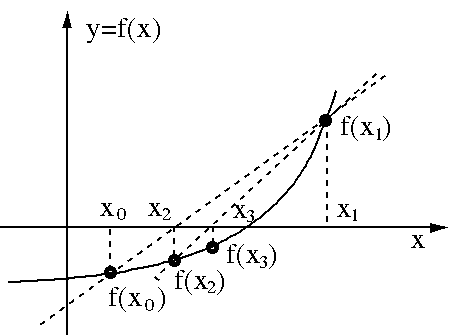
\includegraphics[scale=.5]{secant_method.png}
	\end{center}
	\caption{Geometric Interpretation of Secant Method in $\R$}
\end{figure}

\begin{theorem}(Convergence of Secant Method)
Suppose that $f$ is a real-valued function, defined and continuously differentiable on an interval $I = [\xi - h, \xi + h]$, $h > 0$, with center point $\xi$. Suppose further that $f(\xi) = 0$, $f'(\xi) \neq 0$. Then, the sequence $(x_k)$ defined by the secant method converges at least linearly to $\xi$ provided that $x_0$ and $x_1$ are sufficiently close to $\xi$. 
\end{theorem}

\begin{proof}
Without loss of generality, assume that $\alpha = f'(\xi) > 0$ in a small neighborhood of $\xi$. We'll choose this neighborhood such that
\begin{equation}
	0 < \frac{3}{4}\alpha < f'(x) < \frac{5}{4}\alpha
\end{equation}
for all $x$ in the interval.

Recall that the secant method is defined by 
\begin{equation}
	x_{k+1} = x_k - f(x_k) \frac{x_k - x_{k-1}}{f(x_k) - f(x_{k-1})}
\end{equation}

We can repeatedly use the mean value theorem to approximate each of these terms. First observe that
\begin{equation}
	\frac{f(x_k) - f(\xi)}{x_k - \xi} = f'(\eta_k)
\end{equation}
for some $\eta_k$ between $x_k$ and $\xi$. Since $f(\xi) = 0$, this equation implies that
\begin{equation}
	f'(x_k) = f'(\eta_k)(x_k - \xi)
\end{equation}
Next observe that
\begin{equation}
	\frac{f(x_k) - f(x_{k-1})}{x_k - x_{k-1}} = f'(\theta_k) 
\end{equation}
for some $\theta_k$ between $x_k$ and $x_{k-1}$. Therefore, we can put these pieces together to observe that,
\begin{equation}
	_{k+1} = x_k - \frac{f'(\eta_k)(x_k - \xi)}{f'(\theta_k)}
\end{equation}
To show convergence, we can compare successive error terms.
\begin{align*}
	E_{k+1} &= x_{k+1} - \xi \\
	&= E_k - \frac{f'(\eta_k)}{f'(\theta_k)}E_k  \\
	&= \left( 1 - \frac{f'(\eta_k)}{f'(\theta_k)} \right) E_k
\end{align*}
Therefore
\begin{align*}
	\frac{E_{k+1}}{E_k} &= 1 - \frac{f'(\eta_k)}{f'(\theta_k)} \\
	&< 1 - \frac{5\alpha/4}{3\alpha/4} \\
	&= \frac{2}{3} \\
	&< 1
\end{align*}	
Therefore the secant method converges at least linearly. 
\end{proof}

\section{Solution of systems of linear equations}

\subsection{LU Decomposition}

\subsection{Least Squares}
Given a system of equations $Ax = b$, the least squares problem is
\begin{equation}
	\min_{x \in \R^n} \norm{Ax - b}^2_2 
\end{equation}
We can expand the objective function out as
\begin{align*}
	\norm{Ax - b}^2_2 &= (Ax - b)^T (Ax - b) \\
	&= x^T A^T A x - 2 b^T A x + b^T b 
\end{align*}
To find the $x$ that minimizes this expression we find the $x$ that satisfies $\nabla_x F = 0$. That is
\begin{equation}
	\nabla_x F = 0 = 2 A^T A x - 2 A^T b
\end{equation}
Therefore the minimizer is $x = (A^T A)^{-1} A^T b$. $(A^T A)^{-1} A^T$ is called the pseudo-inverse of $A$. If $A$ is square and invertible, then the pseudo-inverse equals $A^{-1}$.

\subsection{Gram-Schimdt Orthogonalization}
Algorithm: Denote the columns of $A$ by $a_i$. 
\begin{enumerate}
	\item $q_1 = a_1$. Then normalized by $q_1 = \frac{q_1}{\norm{q_1}}$.
	\item $q_2 = a_2 - \inp{q_1}{a_2}q_1$. Then normalize by $q_2 = \frac{q_2}{\norm{q_2}}$. It's simple to verify that $q_2 \perp q_1$. 
	\item For an arbitrary $k$, $q_k = a_k - \inp{a_k}{q_1}q_1 - \inp{a_k}{q_2}q_2 - \ldots - \inp{a_k}{q_{k-1}}q_{k-1}$. Then normalize by $q_k = \frac{q_k}{\norm{q_k}}$.
\end{enumerate}

We can observe the following properties:
\begin{enumerate}
	\item $\norm{q_i} = 1$ (this follows directly)
	\item $q_i \perp q_j$ for all $i \neq j$
	\item $q_k \in span(a_1, \ldots, a_k)$ and $a_k \in span(q_1, \ldots, q_k)$ so that $span(a_1, \ldots, a_k) = span(q_1, \ldots, q_k)$.
\end{enumerate}

[[Write proof for 2]].

\subsection{QR Factorization}
\begin{definition}(Unitary Matrix)
A matrix $Q = [q_1 \ldots q_n] \in \R^{m\times n}$ is unitary if and only if $\inp{q_i}{q_j} = \delta_{ij}$.
\end{definition}

Observations about this definition:
\begin{enumerate}
	\item $Q^T Q = I$
	\item If $Q$ is square, then $Q^T = Q^{-1}$.
\end{enumerate}

To calculate the $QR$ decomposition, we can find $Q$ by using the Gram-Schmidt process. Then $R$ can be found as
\begin{equation}
	R = 
	\begin{pmatrix}
	\inp{e_1}{a_1} & \inp{e_1}{a_2} & \inp{e_1}{a_3} & \hdots \\
	0 & \inp{e_2}{a_2} & \inp{e_2}{a_3} & \hdots \\
	0 & 0 & \inp{e_3}{a_3} & \hdots \\
	\vdots & \vdots & \vdots & \ddots
	\end{pmatrix}
\end{equation}

\subsubsection{Application to Least Squares}
Suppose that we can write $A = QR$, where $A \in \R^{ m \times n}$, $Q \in \R^{ m \times n}$ and unitary, and $R \in \R^{n \times n}$ and upper triangular. Then the least squares solution to $Ax = b$ is given by
\begin{align*}
x &= (A^T A)^{-1} A^T b \\
&= (R^T Q^T Q R)^{-1} R^T Q^T b \\
&= (R^T R)^{-1} R^T Q^T b \\
\implies (R^T R) x &= R^T Q^T b \\
R x &= Q^T b \tag{assume $R$ is invertible (i.e. no zeros on the diagonal)}
\end{align*}
We can then solve for $x$ using back substitution, which is $\mathcal{O}(n^2)$.


\subsection{Norms and Condition Numbers}
\begin{definition}(Norm)\label{norm}
Suppose that $\mathcal{V}$ is a linear space over the field $\R$. The \textit{nonnegative} real-valued function $\norm{\cdot}$ is a norm on $\mathcal{V}$ if the following axioms are satisfied: Fix $v \in \mathcal{V}$
\begin{enumerate}
	\item Positivity: $\norm{v} = 0$ if and only if $v = 0$
	\item Scale Preservation: $\norm{\alpha v} = |\alpha| \norm{v}$ for all $\alpha \in \R$
	\item Triangle Inequality: $\norm{v + w} \leq \norm{v} + \norm{w}$.
\end{enumerate}
\end{definition}

\begin{example}(Examples of Norms)
\begin{enumerate}
	\item 1-norm:
	\begin{equation}
		\norm{v}_1 = \sum_{i=1}^n |v_i| = |v_1| + \cdots + |v_n|
	\end{equation}
	\item 2-norm:
	\begin{equation}
		\norm{v}_2 = \left( \sum_{i=1}^n v_i^2 \right)^{\frac{1}{2}} = \sqrt{v_1^2 + \cdots + v_n^2} = \sqrt{v^T v}
	\end{equation}
	\item $\infty$-norm
	\begin{equation}
		\norm{x}_{\infty} = \max_{i=1, \ldots, n} |v_i|
	\end{equation}
	\item $p$-norm
	\begin{equation}
		\norm{v}_p = \left( \sum_{i=1}^n |v_i|^p \right)^{\frac{1}{p}}
	\end{equation}
	For the $p$-norm, proving the triangle inequality follows from the Minkowski's inequality.
\end{enumerate}
\end{example}

\begin{definition}(Operator Norm)
Let $A$ be an $m \times n$ matrix. That is, $A$ is a linear transformation form $\R^n$ to $\R^m$. Then the operator norm (or subordinate matrix norm) of $A$ is
\begin{equation}
	\norm{A}_{p,q} = \sup_{x \in \R^n, x\neq 0} \frac{\norm{Ax}_q}{\norm{x}_p}.
\end{equation}
\end{definition}

Observations about this definition:
\begin{enumerate}
	\item It's easy to check that this definition of the operator norm satisfies the properties of a norm given in Definition \ref{norm}. For the triangle inequality, observe that
	\begin{align*}
		&\norm{(A + B)x}_p \leq \norm{Ax}_p + \norm{Bx}_p \tag{from Minkowski's inequality} \\
		\implies & \frac{\norm{(A + B)x}_p}{\norm{x}_p} \leq \frac{\norm{Ax}_p}{\norm{x}_p} + \frac{\norm{Bx}_p}{\norm{x}_p}
	\end{align*}
	Taking the supremum of both sides over $x$ shows that $\norm{A + B}_p \leq \norm{A}_p + \norm{B}_p$.
	\item The definition immediately implies that for an arbitrary $x \in \mathbb{R}^n$, $x \neq 0$, 
	\begin{equation}
		\norm{Ax}_q \leq \norm{A}_{p,q} \norm{x}_p
	\end{equation}
	We can generalize this inequality to claim that
	\begin{equation}
		\norm{AB} \leq \norm{A} \norm{B}
	\end{equation}
	for conformable matrices $A, B$. Indeed, fix $0 \neq x \in R^n$. Then
	\begin{equation}
		\norm{ABx} \leq \norm{A} \norm{Bx} \leq \norm{A}\norm{B}\norm{x}
	\end{equation}
	We can divide all inequalities by $\norm{x}$ to see that for all $x \neq 0$,
	\begin{equation}
		\frac{\norm{ABx}}{\norm{x}} \leq \norm{A}\norm{B}
	\end{equation}
	Taking the supremum over $x$ on the left hand side shows that $\norm{AB} \leq \norm{A} \norm{B}$.
\end{enumerate}

\begin{theorem}(The $1$-norm of a matrix is the largest absolute-value column sum)
Let $A \in \R^{m \times n }$ and denote the columns of $A$ by $a_j$, $j=1, \ldots, n$. Then $\norm{A}_1 = \max_{j=1, \ldots, n} \sum_{i=1}^{m} |a_{ij}| =  \max_{j=1, \ldots, n} \norm{a_j}$.
\end{theorem}
\begin{proof}
Fix $x \in \R^n$. Let $C = \max_{j=1, \ldots, n} \sum_{i=1}^{m} |a_{ij}|$. First consider the product $A\cdot x$. The $i$th element is $\sum_{j=1}^n a_{ij} x_j$. Then
\begin{align*}
	\norm{Ax}_1 &= \sum_{i=1}^m |(Ax)_i | = \sum_{i=1}^m |\sum_{j=1}^n a_{ij} x_j| \\
	&\leq \sum_{i=1}^m \sum_{j=1}^n |a_{ij}| |x_j| \tag{triangle inequality} \\
	&= \sum_{j=1}^n |x_j| \left(\sum_{i=1}^m |a_{ij}| \right) \tag{interchange order of summation, assumed finite} \\
	&\leq C \norm{x}_1
\end{align*}
Therefore $\frac{\norm{Ax}_1}{\norm{x}_1} \leq C$ for all $x$. Next, we find an $x$ such we achieve equality with $C$. Call index $J$ the index such that $\norm{a_J}_1 = C = \max_{j=1, \ldots, n} \sum_{i=1}^{m} |a_{ij}|$. Then let $e_J$ be the $n$-vector of zeros with a $1$ in the $J$th entry. Clearly $\norm{e_J}_1 = 1$. But then
\begin{equation}
 	\norm{A e_J}_1 = \norm{a_J}_1 = C
\end{equation} 
In sum, we first showed that for all $x \in \R^n$
\begin{equation}
	\frac{\norm{Ax}_1}{\norm{x}_1} \leq C
\end{equation}
We then found an $x \in \R^n$ such that $\frac{\norm{Ax}_1}{\norm{x}_1} = C$. Therefore 
\begin{equation}
	\norm{A}_1 = \sup_{x \in \R^n, x\neq 0} \frac{\norm{Ax}_1}{\norm{x}_1} = C = \max_{j=1, \ldots, n} \sum_{i=1}^{m} |a_{ij}| =  \max_{j=1, \ldots, n} \norm{a_j}
\end{equation}
\end{proof}

\begin{theorem}(The $\infty$-norm of a matrix is the largest absolute-value row sum)
Let $A \in \R^{m \times n }$ and denote the rows of $A$ by $b_i$, $i=1, \ldots, m$. Then $\norm{A}_{\infty} = \max_{i=1, \ldots, m} \sum_{j=1}^{n} |a_{ij}| =  \max_{i=1, \ldots, m} \norm{b_i}$.
\end{theorem}
\begin{proof}
Fix $x \in \R^n$. Let $C = \max_{i=1, \ldots, m} \sum_{j=1}^{n} |a_{ij}|$.
\begin{align*}
	\norm{Ax}_{\infty} &= \max_{i=1,\ldots,m} |\sum_{j=1}^n a_{ij} x_j| \\
	&\leq \max_{i=1,\ldots,m} \sum_{j=1}^n |a_{ij}| |x_j| \tag{by the triangle inequality} \\
	&\leq  \max_{i=1,\ldots,m} \sum_{j=1}^n |a_{ij}| \norm{x}_{\infty} \tag{since $|x_j| \leq \norm{x}_{\infty}$ for all $j$}\\
	&= C \norm{x}_{\infty}
\end{align*}

Next, we find an $x$ such we achieve equality with $C$. Call $I$ the index for which $\norm{b_I}_\infty = C$. Define
\begin{equation}
	x_j = 
	\begin{cases} 
      1 & a_{Ij} > 0 \\
      -1 & a_{Ij} < 0
   \end{cases}
\end{equation}
Observe that $\norm{x}_\infty = 1$. Then
\begin{align*}
	|A\cdot x|_I &= |b_I^T \cdot x| \\
	&=  |\sum_{j=1}^m a_{Ij} x_j | \\
	&= |\sum_{j=1}^m a_{Ij}| \\
	&= C
\end{align*}
We then found an $x \in \R^n$ such that $\frac{\norm{Ax}_\infty}{\norm{x}_\infty} = C$. Therefore 
\begin{equation}
	\norm{A}_\infty = \sup_{x \in \R^n, x\neq 0} \frac{\norm{Ax}_\infty}{\norm{x}_\infty} = C = \max_{i=1, \ldots, m} \sum_{j=1}^{n} |a_{ij}| =  \max_{i=1, \ldots, m} \norm{b_i}
\end{equation}
\end{proof}

\begin{theorem}(The $2$-norm of a symmetric positive definite matrix is the maximum absolute value of its eigenvalues)
Let $A$ be a positive definite $n \times n$ matrix. Then 
\begin{equation}
	\norm{A}_2 = \max_{i=1,\ldots, n} |\lambda_i|
\end{equation}
\end{theorem}
\begin{proof}
Since $A$ is positive definite, $A$ has $n$ distinct eigenvalues, which implies that it has $n$ linearly independent eigenvectors. Therefore, for an arbitrary $x \in \R^n$, we can write $x$ as a linearly combination of the eigenvectors $x_1$, $\ldots$, $x_n$. Then
\begin{align*}
	x &= c_1 x_1 + \cdots + c_n x_n \\
	A x &= c_1 A x_1 + \cdots + c_n A x_n \\
	&= c_1 \lambda_1 x_2 + \cdots + c_n \lambda_n x_n 
\end{align*}
We can normalize the eigenvectors of $A$ so that $x_i^T x_i = 1$. Then $\norm{Ax}_2 = \sqrt{\sum_{i=1}^n c_i^2 \lambda_i^2}$ and $\norm{x}_2 = \sqrt{\sum_{i=1}^n c_i^2}$. Therefore 
\begin{equation}
	\frac{\norm{Ax}_2}{\norm{x}_2} = \sqrt{\frac{\sum_{i=1}^n c_i^2 \lambda_i^2}{\sum_{i=1}^n c_i^2}} \leq \max_i |\lambda_i| = |\lambda_I|
\end{equation}
Now we'll find an $x$ such that we actually achieve equality. Call $I$ the index of the maximum absolute value of an eigenvalue. Then, consider the eigenvector associated with this eigenvalue, called $x_i$. Then
\begin{equation}
	\frac{\norm{Ax_I}_2}{\norm{x_I}_2} = \frac{|\lambda_I|\norm{x_I}}{\norm{x_I}} = |\lambda_I|
\end{equation}
This shows that $\norm{A}_2 =  \max_i |\lambda_i|$.
\end{proof}

\begin{theorem}(The $2$-norm of a matrix $A_{m \times n}$ equals its largest singular value)
Let $A$ be an $m \times n$ matrix and denote the eigenvalues of the matrix $B = A^TA$ by $\lambda_i$, $i=1,\ldots, n$. Then 
\begin{equation}
	\norm{A}_2 = \max_i \sqrt{\lambda_i}
\end{equation}
The square roots of the (nonnegative) eigenvalues of $A^TA$ are referred to as the singular values of $A$.
\end{theorem}

\subsubsection{Conditioning}
Conditioning helps us quantify the sensitivity of the output to perturbations of the input. In what follows, let $f$ be a mapping from a subset $D$ of a normed linear space $\mathcal{V}$ to another normed linear space $\mathcal{W}$. 
\begin{definition}(Absolute Condition Number)
\begin{equation}
	Cond(f) = \sup_{x,y \in D, x\neq y} \frac{\norm{f(x) - f(y)}}{\norm{x - y}}
\end{equation}
\end{definition}

\begin{definition}(Absolute Local Condition Number)
\begin{equation}
	Cond_x(f) = \sup_{x + \delta x \in D, \delta x \neq 0} \frac{\norm{f(x + \delta x) - f(x)}}{\norm{\delta x}}
\end{equation}
\end{definition}

The previous two definitions depend on the magnitudes of $f(x)$ and $x$. In applications, it's often better to rescale as follows
\begin{definition}(Relative Local Condition Number)
\begin{equation}
	cond_x(f) = \sup_{x + \delta x \in D, \delta x \neq 0} \frac{\norm{f(x + \delta x) - f(x)} / \norm{f(x)}}{\norm{\delta x} / \norm{x}}
\end{equation}
\end{definition}

\textbf{In these definitions, if $f$ is differentiable then we can replace the differences with the appropriate derivatives.} 

\begin{example}(Example of condition numbers)
Let $D$ be a subinterval of $[0, \infty)$ and $f(x) = \sqrt{x}$. Then $f'(x) = \frac{1}{2 \sqrt{x}}$. 
\begin{enumerate}
	\item If $D = [1,2]$, then $Cond(f) = \frac{1}{2}$.
	\item If $D = [0, 1]$, then $Cond(f) = \infty$.
	\item If $D = (0, \infty)$, then the the absolute local condition number of $f$ at $x \in D$ is 
	\begin{equation}
		Cond_x(f) = \frac{1}{2 \sqrt{x}}
	\end{equation}
	Thus as $x \to $, $Cond_x(f) \to \infty$, and as $x \to \infty$, $Cond_x(f) \to 0$.
	\item If $D = (0, \infty)$, then the relative local condition number of $f$ is $cond_x(f) = 1/2$ for all $x \in D$. 
\end{enumerate}
\end{example}

\begin{definition}(Condition Number of a Nonsingular Matrix)
The condition number of a nonsingular matrix $A$ is defined by 
\begin{equation}
	\kappa(A) = \norm{A} \Vert A^{-1} \Vert
\end{equation}
If $\kappa(A) \gg 1$, the matrix is said to be ill-conditioned.
\end{definition}
Observations about this definition:
\begin{enumerate}
	\item $\kappa(A) = \kappa(A^{-1})$ 
	\item For all $A$, $\kappa(A) \geq 1$. This follows because
	\begin{equation}
		1 = \norm{I} = \Vert A A^{-1} \Vert \leq \norm{A} \Vert A^{-1} \Vert
	\end{equation}
	\item The condition number of a matrix is unaffected by scaling all its elements by multiplying by a nonzero constant.
	\item There is a condition number for each norm, and the size of the condition number is strongly dependent on the choice of norm.
\end{enumerate}

\section{Special Matrices}
\subsection{Symmetric Positive Definite Matrices }
\begin{definition}(Symmetric, Positive Definite, spd)
The real matrix $A$ is said to be symmetric if $A = A^T$. A square $n \times n$ matrix is called positive definite if 
\begin{equation}
 	\x^T A \x > 0
\end{equation}
for all $\x \in \R^n$, $\x \neq 0$. 
\end{definition}

\begin{theorem}(Properties of spd matrices)
Let $A$ be an $n \times n$ real, spd matrix. Then
\begin{enumerate}
	\item $a_{ii} > 0$ for all $i=1, \ldots, n$ (the diagonal elements of $A$ are positive). 
	\item $A x_i \ = \lambda_i x_i \implies \lambda_i \in \R_{>0}, \x \in \R^n \setminus \{0\}$ (the eigenvalues of $A$ are real and positive, and the eigenvectors of $A$ belong to $\R^n \setminus \{0\}$).
	\item $x_i \perp x_j$ if $\lambda_i \neq \lambda_j$ (the eigenvectors of distinct eigenvalues of $A$ are orthogonal)
	\item $\det(A) > 0$ (the determinant of $A$ is positive)
	\item Every submatrix $B$ of $A$ obtained by deleting any set of rows and the corresponding set of columns from $A$ is symmetric and positive definite (in particular, every principal submatrix is positive definite). 
\end{enumerate}
\end{theorem}

\begin{proof}
We prove each claim in the theorem as follows
\begin{enumerate}
	\item Let $e_i$ be the $i$th canonical basis vector in $\R^n$. Then
	\begin{equation}
		a_{ii} = e_i^T A e_i > 0
	\end{equation}
	since $A$ is pd. A few observations: this only relies on $A$ being pd. $e_i^T A$ picks out the $i$th row of $A$. $A e_i$ picks out the $i$th column of $A$. 
	\item We'll first show that the eigenvalues of $A$ are real. Suppose $\lambda$, $\x$ are an eigenvalue/vector pair of $A$. Thus $A \x = \lambda \x$. We can conjugate this equation to find that $\bar A \bar \x = A \bar \x = \bar \lambda \bar x$ (thus complex eigenvalues of real valued matrices come in conjugate pairs). Then
	\begin{align*}
	\x^T A \bar\x &= \bar \lambda \x^T \bar \x \\
	\x^T A^T \bar\x &= (A\x)^T \bar \x = \lambda \x^T \bar \x
	\end{align*}
	Since $A = A^T$, we know that $\lambda \x^T \bar \x = \lambda \x^T \bar \x$. As long as $\x \neq 0$, then $\x^T \bar \x \neq 0$. Therefore $\bar \lambda = \lambda$, which shows $\lambda \in \R$. 

	The fact that the eigenvector associated with $\lambda$ has real elements follows by noting that all elements of the singular matrix $A - \lambda I$ are real numbers. Therefore, the columns of $A - \lambda I$ are linearly dependent in $\R^n$. Hence there exists an $\x \in \R^n$ such that $(A - \lambda I)\x = 0$. 

	This proof only requires that $A$ is symmetric -- therefore any real, symmetric matrix has real eigenvalues/vectors. 

	Next we'll show the eigenvalues of $A$ are positive. Suppose $\lambda$, $\x$ are an eigenvalue/vector pair of $A$. Then
	\begin{equation}
		0 < \x^T A \x = \lambda \x^T \x
	\end{equation}
	Since $\x \neq 0$ and $\x^T \x$ is positive (it's actually the squared $2$-norm of $\x$), then $\lambda > 0$. Note that this part of the proves requires $A$ be pd.

	\item Let $\lambda_i, \lambda_j$ be distinct eigenvalues of $A$, and $\x_i, \x_j$ the corresponding eigenvectors. Then
	\begin{align*}
		\x_i^T A \x_j &= \lambda_j \x_i^T \x_j \\
		\x_i^T A^T \x_j &= (A\x_i)^T x_j = \lambda_i \x_i^T \x_j 
	\end{align*}
	Since $A$ is symmetric, these two string of equalities must be equal. We can subtract them to find that 
	\begin{equation}
		(\lambda_i - \lambda_j)\x_i^T \x_j = 0
	\end{equation}
	Since we assumed $\lambda_i \neq \lambda_j$, then it must be that $\x_i^T \x_j$. Therefore $x_i \perp x_j$. This proof again only relies on the symmetry of $A$. 
 	which is the product of the diagonal elements of the matrix (the eigenvalues). 
	\item This follows from the fact that the determinant of $A$ is equal to the product of its eigenvalues. Or, we can write $A$ in terms of its eigenvalue decomposition. Thus
	\begin{equation}
		A = X \Lambda X^{-1}
	\end{equation}
	Therefore
	\begin{equation}
		\det(A) = \det(X) \det(\Lambda) \det(X)^{-1} = \det(\Lambda) 
 	\end{equation}Or, we can write $A$ in terms of its eigenvalue decomposition. Thus
	\begin{equation}
		A = X \Lambda X^{-1}
	\end{equation}
	Therefore
	\begin{equation}
		\det(A) = \det(X) \det(\Lambda) \det(X)^{-1} = \det(\Lambda) 
 	\end{equation}
	\item Let $I \subset \{1,2,\ldots, n\}$ be a subset of indices and let $B = A_{II}$. $A$ is symmetric, so that $A_{II} = A_{II}^T$. Therefore $B$ is symmetric. Let $x \in \R^n$ and define a vector $y$ that is $0$ for the indices not included in $I$ and follows the value of $x$ for the indices included in $I$. Therefore, $x^TBx = y^TAy > 0$ since $A$ is pd. 
\end{enumerate}
\end{proof}

\subsection{Cholesky Factorization}

\begin{theorem}
If $A$ is spd, then there exists a lower diagonal matrix $L$ such that $A = L L^T$. This is called the Cholesky decomposition. 
\end{theorem}

\begin{algorithm}
  \caption{Cholesky Factorization}
  \begin{algorithmic}[ht]
    \Require{$A \in \R^{n \times n}$, SPD}
    \Let{$L_1$}{$\sqrt{a_{11}}$}
    \For{$k \gets 2, 3, \ldots, n$}
    	\State Solve $L_{k-1} l_k = a_k$ for $l_k$
    	\Let{$l_{kk}$}{$\sqrt{a_{kk} - l_k^T l_k}$}
    	\Let{$L_k$}{$\begin{pmatrix} L_{k-1} & 0 \\ l_k^T & l_{kk} \end{pmatrix}$}
    \EndFor
  \end{algorithmic}
\end{algorithm}
Notation:
\begin{itemize}
	\item $L_{k-1}$: the first $k-1 \times k-1$ upper left corner of $L$
	\item $a_k$: the first $k-1$ entries in column $k$ of $A$
	\item $l_k$: the first $k-1$ entries in column $k$ of $L^T$ [[?]]
	\item $a_{kk}, l_{kk}$: the $kk$ entries of $A$ and $L$, respectively
\end{itemize}

\subsection{Banded Matrices and Differential Equations}
Consider the two-point boundary value problem
\begin{equation}
	u'' + 2u' = -1, \quad u(x=0)=0, u(x=1)= 0
\end{equation}
where $x\in [0,1]$.

Define a sequence of grid points $\{x_i\}_{i=0}^{N+1}$. We can approximate the derivative of $u$ at each point on the grid as follows
\begin{align*}
	u'(x_j) &= \lim_{\delta \to 0} \frac{u(x_j + \delta) - u(x_j - \delta)}{2\delta} \\
	&\approx \frac{u(x_{j-1}) - u(x_{j+1})}{2\Delta x}
\end{align*}
where we use the centered difference quotient of order $2$. Similarly, we can approximate the second derivative of $u$ each each point in the domain as
\begin{align*}
	u''(x_j) &= \lim_{\delta \to 0} \frac{u'(x_j + \delta) - u'(x_j - \delta)}{2\delta} \\
	&\approx \frac{u'(x_{j+1}) - u'(x_{j-1})}{2\Delta x} \\
	&= \frac{\frac{u(x_{j+2}) - u(x_j)}{2\Delta x} - \frac{u(x_j) - u(x_{j-2})}{2\Delta x}}{2\Delta x} \\
	&= \frac{u(x_{j+2}) - 2u(x_j) + u(x_{j-2})}{4\Delta x}
\end{align*}
Let's instead use the grid points adjacent to $x_j$:
\begin{equation}
	u''(x_j) \approx \frac{u(x_{j+1}) - 2u(x_j) + u(x_{j-1})}{\Delta x}
\end{equation}
Then, going back to the initial differential equation, for $x_j$, we have
\begin{equation}
	\frac{u(x_{j+1}) - 2u(x_j) + u(x_{j-1})}{\Delta x} + 2 \frac{u(x_{j-1}) - u(x_{j+1})}{2\Delta x} = -1
\end{equation}
Let
\begin{equation}
	U = 
	\begin{bmatrix}
	u(x_1) \\ u(x_2) \\ \vdots \\ u(x_N)
	\end{bmatrix}
\end{equation}
and let $u_i = u(x_i)$. In this notation, the differential equation at $x_j$ can be written as
\begin{equation}
	\frac{u_{j+1} - 2u_j + u_{j-1}}{\Delta x^2} + \frac{u_{j-1} - u_{j+1}}{\Delta x} = -1
\end{equation}
We can put these equations together into a matrix. Each row will only have $3$ non-zero entries at $j-1$, $j$, and $j+1$. Thus the $j$th row is
\begin{equation}
	\begin{pmatrix}
	0 & 0 & \hdots & \frac{1}{\Delta x^2} + \frac{1}{\Delta x} & \frac{-2}{\Delta x^2} & \frac{1}{\Delta x^2} - \frac{1}{\Delta x} & 0 & 0 & \hdots
	\end{pmatrix}
\end{equation}
Thus stacking these rows together will give a tridiagonal matrix. Call this matrix $A$. Then we have that
\begin{equation}
	AU = \bm{-1}
\end{equation}

\section{Simultaneous nonlinear equations}

\subsection{Analysis Preliminaries}
\begin{definition}(Cauchy Sequence)
A sequence $(\x^{(k)}) \subset \R^n$ is called a Cauchy sequence in $\R^n$ if for any $\e > 0$ there exists a positive integer $k_0 = k_0(\e)$ such that
\begin{equation}
	\norm{\x^{(k)} - \x^{(m)}}_{\infty} < \e \quad \forall k, m \geq k_0(\e)
\end{equation}
\end{definition}

\begin{remark}
$\R^n$ is \textbf{complete} in the sense that every Cauchy sequence $(\x^{(k)})$ converges to some $\xi \in \R^n$. 
\end{remark}

\begin{definition}(Continuous function)
Let $D \subset \R^n$ be nonempty and $f: D \to \R^n$. Given $\xib \in D$, $f$ is continuous at $\xib$ if for every $\e > 0$, there exists a $\delta = \delta(\e) > 0$ such that for every $\x \in B(\xib; \delta) \cap D$
\begin{equation}
 	\norm{f(\x) - f(\xib)}_\infty < \e
 \end{equation} 
\end{definition}

\begin{lemma}
Let $D \subset \R^n$ be nonempty and $f: D \to \R^n$ be defined and continuous on $D$. If $(\x^{(k)}) \subset D$ converges in $\R^n$ to $\xib \in D$, then $f(\x^{(k)})$ also converges to $f(\xib)$. 
\end{lemma}

We want to find a vector $\x\in \R^n$ such that $f(\x) = 0$.

\begin{example}
Consider the linear system
\begin{equation}
	Ax = b
\end{equation}
Then $A: \R^n \to \R^m$. Let $f(\bm x) = A\x - b$.
\end{example}

\begin{example}
Let 
\begin{equation}
	f = 
	\begin{bmatrix}
	x_1^2 + x_2^2 - 1 \\
	5x_1^2 + 21x_2^2 - 9
	\end{bmatrix}
\end{equation}
Note that $x_1^2 + x_2^2 = 1$ is the $0$ level set of $f$, and is the unit circle. $5x_1^2 + 21x_2^2 = 9$ is the $0$ level set of $f$ and is an ellipse. 

This function has four zeros
\begin{equation}
	\begin{bmatrix}
	x_1 \\ x_2
	\end{bmatrix}
	=
	\begin{bmatrix}
	\pm \sqrt{3}/2 \\
	\pm \frac{1}{2}
	\end{bmatrix}
\end{equation}
\end{example}

\subsection{Simultaneous iteration}

\begin{example}

\end{example}


\begin{definition}(Lipschitz condition, constant, and contraction)
Let $D$ be a closed subset of $\R^n$ and $g: D \to D$. If there exists a positive constant $L$ such that
\begin{equation}
	\norm{g(x) - g(y)}_\infty \leq L \norm{x - y}_\infty
\end{equation}
for all $x, y \in D$, then $g$ satisfies the Lipschitz condition on $D$ in the $\infty$-norm. $L$ is called the Lipschitz constant. If $L \in (0,1)$, then $g$ is called a contraction on $D$ in the $\infty$-norm. 
\end{definition}

Observations about this definition:
\begin{itemize}
	\item Any function $g$ that satisfies the Lipschitz condition on $D$ is continuous on $D$ (to see this, set $\delta = \frac{\e}{L}$). 
	\item If $g$ satisfies the Lipschitz condition on $D$ in the $\infty$-norm, then it also does in the $p$-norm for $p \in [1, \infty)$ and vice-versa. However the size of $L$ depends on the choice of norm. 
\end{itemize}

\begin{theorem}(Contraction Mapping Theorem in $\R^n$)
Suppose $D$ is a closed subset of $\R^n$ and $g: \R^n \to \R^n$ is defined on $D$, and $g(D) \subset D$. Suppose further that $g$ is a contraction on $D$ in the $\infty$-norm. Then,
\begin{enumerate}
	\item $g$ has a unique fixed point $\xib \in D$
	\item The sequence $(\x^{(k)})$ defined by $\x^{(k+1)} = g(\x^{k})$ converges to $\xib$ for any starting value $x^{(0)} \in D$.
\end{enumerate}
\end{theorem}

\begin{proof}
The proof has three parts:
\begin{enumerate}
	\item First prove uniqueness, assuming existence of a fixed point.
	\item Prove the iteration generates a Cauchy sequence (then convergence to some $\xib$ follows from the completeness of the space).
	\item Show $\xib$ is indeed the fixed point.
\end{enumerate}

Uniqueness: Suppose $\xib, \bm \eta$ are both fixed points of $g$ in $D$. Then,
\begin{align*}
	\norm{\xib - \bm \eta}_\infty &= \norm{g(\xib) - g(\bm \eta)} \tag{$\xib, \bm \eta$ are fixed points} \\
	&\leq L \norm{\xib - \bm \eta}_\infty \tag{$g$ is a contraction on $D$}
\end{align*}
We can rearrange this to see that $(1-L)\norm{\xib - \bm \eta}_\infty \leq 0$. By assumption, $L\in (0,1)$, and the norm of a quantity is always weakly positive. Therefore, $\norm{\xib - \bm \eta}_\infty = 0$ which implies $\xib = \bm \eta$. 

Convergence: Assuming $g$ has a fixed point $\xib \in D$, the sequence $\x^{(k+1)} = g(\x^{k})$ will converge to $\xib$ for any $\x^{(0)} \in D$. This follows because
\begin{equation}
	\norm{\x^{(k)} - \xib}_\infty \leq L^k \frac{1}{1-L} \norm{\x^{(1)} - \x^{(0)}}_\infty
\end{equation}
Since $L \in (0,1)$, $\lim_{k\to\infty} L^k = 0$, and therefore
\begin{equation}
	\lim_{k \to \infty} \norm{\x^{(k)} - \xib}_\infty = 0
\end{equation}

Existence: First observe that if $\x^{(0)}$ belongs to $D$, then $\x^{(k+1)} = g(\x^{k}) \in D$ for all $k \geq 1$ since $g(D) \subset D$ (this is important since the proof relies on $g$ being a contraction on $D$). Next, consider the distance between two adjacent terms on the sequence $\x^{(k+1)} = g(\x^{k})$
\begin{align*}
	\norm{\x^{(k)} - \x^{(k-1)}}_\infty &= \norm{g(\x^{(k-1)}) - g(\x^{(k-2)})}_\infty \tag{definition of $g$} \\
	&\leq L \norm{\x^{(k-1)} - \x^{(k-2)}}_\infty \tag{$g$ is a contraction on $D$} \\
	&\leq L^{k-1} \norm{\x^{(1)} - \x^{(0)}}_\infty \tag{induction}
\end{align*}

Now, fix positive integers $m,k$ such that $m > k$. Then
\begin{align*}
	\norm{\x^{(m)} - \x^{(k)}}_\infty &= \norm{\x^{(m)} - \x^{(m-1)} + \x^{(m-1)} + \cdots + \x^{(k-1)} - \x^{(k)}}_\infty \\
	&\leq \norm{\x^{(m)} - \x^{(m-1)}}_\infty + \cdots + \norm{\x^{(k+1)} - \x^{(k)}}_\infty \tag{triangle inequality} \\
	&\leq (L^{m-1} + \cdots + L^k) \norm{\x^{(1)} - \x^{(0)}}_\infty \tag{$g$ a contraction} \\
	&= L^k (L^{m-k-1} + \cdots + 1) \norm{\x^{(1)} - \x^{(0)}}_\infty \\
	&\leq L^k \frac{1}{1-L} \norm{\x^{(1)} - \x^{(0)}}_\infty \tag{geometric series}
\end{align*}

Since $L \in (0,1)$, $\lim_{k\to\infty} L^k = 0$. Therefore, $\x^{(k)}$ is a Cauchy sequence in $\R^n$, that is for all $\e > 0$, there exists a $k_0$ such that 
\begin{equation}
	\norm{\x^{(m)} - \x^{(k)}}_\infty < \e \quad \forall m,k \geq k_0
\end{equation}

Any Cauchy sequence in $\R^n$ is convergent in $\R^n$. Thus, there exists some $\xib \in \R^n$ such that $\xib = \lim_{k \to \infty} \x^{(k)}$. 

$\xib$ is indeed the fixed point: Since $g$ satisfies the Lipschitz condition on $D$, $g$ is continuous on $D$. Therefore, 
\begin{equation}
	\xib = \lim_{k \to \infty} \x^{(k+1)} = \lim_{k \to \infty} g(\x^{(k)}) = g \left( \lim_{k \to \infty} \x^{(k)} \right) = g(\xib)
\end{equation}
therefore $\xib$ is a fixed point of $g$, and observe that $\xib \in D$ since $D$ is closed. 
\end{proof}

\begin{definition}(Jacobian)
Let $g = (g_1, \ldots, g_n)^T : \R^n \to \R^n$ be a function defined and continuous in an (open) neighborhood of $\xib \in \R^n$. Suppose the first partial derivatives of each $g_i$ exist at $\xib$. The Jacobian matrix $J_g(\xib)$ of $g$ at $\xib$ is the $n \times n$ matrix with elements
\begin{equation}
	J_g(\xib)_{ij} = \frac{\partial g_i}{\partial x_j} (\xib) 
\end{equation}
\end{definition}

\begin{theorem}
Let $g = (g_1, \ldots, g_n)^T : \R^n \to \R^n$ be a function defined and continuous on a closed set $D \subset \R^n$. Let $\xib \in D$ be a fixed point of $g$. Suppose the first partial derivatives of each $g_i$ are defined and continuous in some (open) neighborhood $N(\xib) \in D$ of $\xib$, with 
\begin{equation}
	\norm{J_g(\xib)}_\infty < 1  	
\end{equation}
Then there exists $\e > 0$ such that $g (\bar B_\e(\xib)) \subset \bar B_\e(\xib)$, and the sequence $\x^{(k+1)} = g(\x^{k})$ converges to $\xib$ for all $\x^{(0)} \in \bar B_\e(\xib)$ (in other words, the sequence converges to $\xib$ as long as $\x^{(0)}$ is close enough to $\xib$).
\end{theorem}

\begin{example}

\end{example}

\subsection*{Newton's Method}
\begin{definition}(Newton's Method)
	The sequence defined by
	\begin{equation}
		\x^{(k+1)} = \x^{(k)} - [J_f(\x^{(k)})]^{-1} f(\x^{(k)})
	\end{equation}
	where $\x^{(0)} \in \R^n$, is called Newton's method. 
\end{definition}

\begin{theorem}
Suppose $f(\xib) = 0$, that in some (open) neighborhood $N(\xib)$ of $\xib$, where $f$ is defined and continuous, all the second-order partial derivatives of $f$ are defined and continuous, and that the Jacobian matrix $J_f(\x^{(k)})$ of $f$ at the point $\xib$ is nonsingular. Then the sequence defined by Newton's method converges to $\xib$ provided that $\x^{(0)}$ is sufficiently close to $\xib$. 
\end{theorem}


\section{Eigenvalues of Eigenvectors of a symmetric matrix}

Another matrix decomposition is
\begin{equation}
	A = X \Lambda X^{-1}
\end{equation}
where $X$ is a matrix of the eigenvectors and $\Lambda$ is a diagonal matrix with the eigenvalues. 

\subsection{Why we use iteration to calculate eigenvalues/eigenvectors}
We call $\lambda$ an eigenvalue and $x \neq 0$ an eigenvector of $A$ if $Ax = \lambda x$. Thus, $(Ax - \lambda I) = 0$. Therefore, $x \in Null(A - \lambda I)$. Since $x \neq 0$, $A - \lambda I$ has a non-trivial nullspace, so we must have $\det(A - \lambda I) = 0$. This suggests a way to transform an eigenvalue finding problem to a root finding problem. Define
\begin{equation}
	\rho(\lambda) = \det(A - \lambda I)
\end{equation}
Recall that the determinant of a matrix is the product of its eigenvalues. If $A$ is a $n \times n$ real, symmetric matrix, then $\rho(\lambda)$ is an $n$-th order polynomial in $\lambda$, whose roots are the eigenvalues of $A$. 

\begin{theorem}(Abel(-Ruffini) Theorem, or ``No-go Theorem'')
There is no algebraic solution (that is, a solution expressed in terms of radicals) to general polynomial equations of degree five or higher with arbitrary coefficients.  
\end{theorem}

Therefore, there is no finite-number operation procedure that provides an eigenvalue decomposition. 

\subsection{Power Iteration}
\textbf{Find the biggest eigenvalue/vector.}

\begin{algorithm}[ht]
  \caption{Power Iteration}
  \begin{algorithmic}[1]
    \Require{$v^{(0)} =$ some vector with $\norm{v^{(0)}} = 1$}
    \For{$k \gets 1, 2, \ldots$}
	    \Let{$w$}{$Av^{(k-1)}$} \Comment{Apply $A$}
	    \Let{$v^{(k)}$}{$w/ \norm{w}$} \Comment{Normalize}
	    \Let{$\lambda^{(k)}$}{$(v^{(k)})^T Av^{(k)} = \inp{v^{(k)}}{Av^{(k)}}$} \Comment{Rayleigh Quotient}
    \EndFor
  \end{algorithmic}
\end{algorithm}

\begin{theorem}(Convergence of Power Iteration)
Suppose $|\lambda_1|  > |\lambda_2| \geq \ldots \geq |\lambda_n|$ and $q_1^T v^{(0)} \neq 0$. Then the iterates of power iteration satisfy
\begin{align}
	\norm{v^{(k)} - (\pm q_1)} &= \mathcal{O}\left( \left\vert \frac{\lambda_2}{\lambda_1} \right\vert^k \right) \tag{error of eigenvector} \\
	|\lambda^{(k)} - \lambda_1 | &= \mathcal{O}\left( \left\vert \frac{\lambda_2}{\lambda_1} \right\vert^{2k} \right) \tag{error of eigenvalue}
\end{align}
\end{theorem}

\begin{proof}

Convergence of eigenvector: Write $v^{(0)} = v$ as a linear combination of the orthonormal eigenvectors $q_i$:
\begin{equation}
	v = c_1 q_1 + \cdots + c_nq_n
\end{equation}

$v^{(k)}$ is a scalar multiple of $A^k v^{(0)}$. Therefore

\begin{align*}
	v^{(k)} &= \alpha_k A^k v^{(0)} \tag{$\alpha_k$ a normalization constant} \\
	&= \alpha_k \left(\sum_{i=1}^n \lambda_i^k a_i q_i \right) \\
	&= \alpha_k \lambda_1^k \left( c_1q_1 + c_2 \left(\frac{\lambda_2}{\lambda_1} \right)^k q_2 + \ldots + c_n \left(\frac{\lambda_n}{\lambda_1} \right)^k q_n \right) \\
\end{align*}
We can choose $\alpha_k$ such that $\alpha_k \lambda_1^k$ is 1. Therefore, $c_1 q_1$ is dominating (as long as $c_1 \neq 0$). The other terms are of order $\mathcal{O}\left( \left\vert \frac{\lambda_2}{\lambda_1} \right\vert^k \right)$.

Convergence of eigenvalue: see proposition below.

\end{proof}

\begin{theorem}(Error of Rayleigh Quotient)
Let $x_1$ be the eigenvector that corresponds to the largest (in absolute value) eigenvalue. If $\norm{x - x_1} = \mathcal{O}(\e)$, then
\begin{equation}
	\left\vert \frac{\inp{x}{Ax}}{\inp{x}{x}}  - \lambda_1 \right\vert = \mathcal{O}(\e^2)
\end{equation}
\end{theorem}
\begin{proof}
\color{Red}{TODO}. 
\end{proof}


\subsection{Inverse Iteration}
\textbf{Find the smallest eigenvalue/vector}. 

\subsection{Simultaneous Iteration}
\textbf{Obtain the full set of eigenvalues/vectors simultaneously.}

\begin{algorithm}[ht]
  \caption{Simultaneous Iteration}
  \begin{algorithmic}[1]
    \Require{$Q^{(0)} = V = I$, a list of vectors $V$, which we choose to be the identity}
    \For{$k \gets 1, 2, \ldots$}
	    \Let{$Z$}{$A \underline Q^{(k-1)}$} \Comment{Apply $A$}
	    \Let{$Z$}{$\underline Q^{(k)} R^{(k)}$} \Comment{$QR$ factorization of $Z$}
	    \Let{$A^{(k)}$}{$(\underline Q^{(k)})^T A \underline Q^{(k)}$}  \Comment{$A^{(k)}_{ii} = \inp{q_i^{(k)}}{Aq_i^{(k)}}$}
    \EndFor
  \end{algorithmic}
\end{algorithm}

Intuitively, 
\begin{equation}
	A^K \cdot V = 
	\begin{bmatrix}
	\sum_i \lambda_i^k c_{1i} \tilde{q_i} &\vert & \sum_i \lambda_i^k c_{2i} \tilde{q_i}&\vert & \cdots
	\end{bmatrix}
\end{equation}
The first column vector will converge to $\tilde{q}_1$. The second vector will converge to $\tilde{q}_1 + \mathcal{O}\left( \left\vert \frac{\lambda_2}{\lambda_1} \right\vert^k \right) \tilde{q}_2$. 

$\underline Q^{(k)}$ will converge to the matrix of eigenvectors:
\begin{equation}
	X = 
	\begin{bmatrix}
	x_1 &|& x_2 &|& \cdots &|&x_n 
	\end{bmatrix}
\end{equation}

$\underline A^{(k)}$ will converge to a diagonal matrix containing the eigenvalues.

\subsection{Shifted Power Iteration}
\textbf{Find the eigenvalue close to a specific number.}

\subsection{QR Algorithm}
The $QR$ can be viewed as a stable procedure for computing $QR$ factorizations of the matrix powers $A$, $A^2$, $A^3$, $\ldots$

\begin{algorithm}[ht]
  \caption{QR Algorithm (without shifts)}
  \begin{algorithmic}[1]
    \Require{$A^{(0)} = A$}
    \For{$k \gets 1, 2, \ldots$}
	    \Let{$Q^{(k)}R^{(k)}$}{$A^{(k-1)}$} \Comment{$QR$ factorization of $A^{(k-1)}$}
	    \Let{$A^{(k)}$}{$R^{(k)}Q^{(k)}$} \Comment{Recombine factors in reverse order}
    \EndFor
  \end{algorithmic}
\end{algorithm}

\subsection{Simultaneous Iteration equivalent to QR Algorithm}
The $QR$ algorithm is equivalent to simultaneous iteration applied to a full set of initial vectors, namely, $\hat Q^{(0)} = I$. Summary of each algorithm:

\subsubsection*{Simultaneous Iteration}
\begin{align}
	\underline Q^{(0)} &= I \tag{initial condition} \\
	Z &= A \underline Q^{(k-1)} \tag{apply $A$}\\
	Z &= \underline Q^{(k)} R^{(k)} \tag{resemblence of normalization, $QR$ factorization of $Z$} \\
	A^{(k)} &= (\underline Q^{(k)})^T A \underline Q^{(k)} \tag{resemblence of Rayleigh quotient}
\end{align}

\subsubsection*{QR Algorithm}
\begin{align}
	A^{(0)} &= A \tag{initial condition}\\
	A^{(k-1)} &= Q^{(k)}R^{(k)} \tag{compute $QR$ factorization}\\
	A^{(k)} &= R^{(k)}Q^{(k)} \tag{reverse order of factors}\\
	\underline Q^{(k)} &= Q^{(1)} Q^{(2)} \cdots Q^{(k)} \tag{definition of $\underline Q^{(k)}$}
\end{align} 
and 
\begin{equation}
	\underline R^{(k)} = R^{(k)} R^{(k-1)} \cdots R^{(1)} \tag{definition of $\underline R^{(k)}$}
\end{equation}

\begin{theorem}(Equivalence of Simultaneous Iteration and the QR Algorithm)
Simultaneous Iteration and the QR Algorithm generate identical sequences of matrices $\underline R^{(k)}, \underline Q^{(k)}, A^{(k)}$. Both give
\begin{align}
	(a): A^{(k)} &= \underline Q^{(k)} \underline R^{(k)} \tag{$QR$ factorization of the $k$th power of $A$}\\
	(b): A^{(k)} &= (\underline Q^{(k)})^T A \underline Q^{(k)} \tag{projection}
\end{align}
\end{theorem}
\begin{proof}
By induction on $k$ (number of iterations). The base case $k=0$ is trivial. 
\begin{enumerate}
	\item $QR$ gives $(a)$: Assume $A^{(k-1)} = \underline Q^{(k-1)} \underline R^{(k-1)}$. The inductive hypothesis for $(b)$ gives that $A^{(k-1)} = (\underline Q^{(k-1)})^T A \underline Q^{(k-1)}$ or that $ \underline Q^{(k-1)} A^{(k-1)} = A \underline Q^{(k-1)}$. Then
	\begin{align*}
		A^{(k)} &= A A^{(k-1)} \tag{decompose to use inductive hypothesis}\\
		&= A \underline Q^{(k-1)} \underline R^{(k-1)} \tag{inductive hypothesis}\\
		&= \underline Q^{(k-1)} A^{(k-1)} \underline R^{(k-1)} \tag{inductive hypothesis from $(b)$}\\
		&= \underline Q^{(k-1)} R^{(k-1)}Q^{(k-1)} \underline R^{(k-1)} \tag{from algorithm} \\
		&= \underline Q^{(k)} \underline R^{(k)} \tag{from definitions of $\underline Q^{(k)}, \underline R^{(k)}$}
	\end{align*}
	\item $QR$ gives $(b)$: Assume $A^{(k-1)} = (\underline Q^{(k-1)})^T A \underline Q^{(k-1)}$. From the relationship $A^{(k-1)} = Q^{(k)}R^{(k)}$ and the fact that $Q^{(k)}$ is orthogonal, we can apply $(Q^{(k)})^T$ to both sides (on the left) to get that $(Q^{(k)})^T A^{(k-1)} = R^{(k)}$. Then
	\begin{align*}
		A^{(k)} &= R^{(k)}Q^{(k)} \\
		&= (Q^{(k)})^T A^{(k-1)} Q^{(k)} \\
		&= (Q^{(k)})^T (\underline Q^{(k-1)})^T A \underline Q^{(k-1)} Q^{(k)} \tag{inductive hypothesis} \\
		&= (\underline Q^{(k)})^T A \underline Q^{(k)} \tag{definition of $\underline Q^{(k)}$}
	\end{align*}
\end{enumerate}
\end{proof}

\end{document}